\documentclass[]{book}
\usepackage{lmodern}
\usepackage{amssymb,amsmath}
\usepackage{ifxetex,ifluatex}
\usepackage{fixltx2e} % provides \textsubscript
\ifnum 0\ifxetex 1\fi\ifluatex 1\fi=0 % if pdftex
  \usepackage[T1]{fontenc}
  \usepackage[utf8]{inputenc}
\else % if luatex or xelatex
  \ifxetex
    \usepackage{mathspec}
  \else
    \usepackage{fontspec}
  \fi
  \defaultfontfeatures{Ligatures=TeX,Scale=MatchLowercase}
\fi
% use upquote if available, for straight quotes in verbatim environments
\IfFileExists{upquote.sty}{\usepackage{upquote}}{}
% use microtype if available
\IfFileExists{microtype.sty}{%
\usepackage{microtype}
\UseMicrotypeSet[protrusion]{basicmath} % disable protrusion for tt fonts
}{}
\usepackage[margin=1in]{geometry}
\usepackage{hyperref}
\hypersetup{unicode=true,
            pdftitle={English 3844: Writing and Digital Media Guidebook},
            pdfauthor={Andy Lautenschlager},
            pdfborder={0 0 0},
            breaklinks=true}
\urlstyle{same}  % don't use monospace font for urls
\usepackage{natbib}
\bibliographystyle{apalike}
\usepackage{longtable,booktabs}
\usepackage{graphicx,grffile}
\makeatletter
\def\maxwidth{\ifdim\Gin@nat@width>\linewidth\linewidth\else\Gin@nat@width\fi}
\def\maxheight{\ifdim\Gin@nat@height>\textheight\textheight\else\Gin@nat@height\fi}
\makeatother
% Scale images if necessary, so that they will not overflow the page
% margins by default, and it is still possible to overwrite the defaults
% using explicit options in \includegraphics[width, height, ...]{}
\setkeys{Gin}{width=\maxwidth,height=\maxheight,keepaspectratio}
\IfFileExists{parskip.sty}{%
\usepackage{parskip}
}{% else
\setlength{\parindent}{0pt}
\setlength{\parskip}{6pt plus 2pt minus 1pt}
}
\setlength{\emergencystretch}{3em}  % prevent overfull lines
\providecommand{\tightlist}{%
  \setlength{\itemsep}{0pt}\setlength{\parskip}{0pt}}
\setcounter{secnumdepth}{5}
% Redefines (sub)paragraphs to behave more like sections
\ifx\paragraph\undefined\else
\let\oldparagraph\paragraph
\renewcommand{\paragraph}[1]{\oldparagraph{#1}\mbox{}}
\fi
\ifx\subparagraph\undefined\else
\let\oldsubparagraph\subparagraph
\renewcommand{\subparagraph}[1]{\oldsubparagraph{#1}\mbox{}}
\fi

%%% Use protect on footnotes to avoid problems with footnotes in titles
\let\rmarkdownfootnote\footnote%
\def\footnote{\protect\rmarkdownfootnote}

%%% Change title format to be more compact
\usepackage{titling}

% Create subtitle command for use in maketitle
\newcommand{\subtitle}[1]{
  \posttitle{
    \begin{center}\large#1\end{center}
    }
}

\setlength{\droptitle}{-2em}
  \title{English 3844: Writing and Digital Media Guidebook}
  \pretitle{\vspace{\droptitle}\centering\huge}
  \posttitle{\par}
  \author{Andy Lautenschlager}
  \preauthor{\centering\large\emph}
  \postauthor{\par}
  \predate{\centering\large\emph}
  \postdate{\par}
  \date{2018-10-08}

\usepackage{booktabs}
\usepackage{amsthm}
\makeatletter
\def\thm@space@setup{%
  \thm@preskip=8pt plus 2pt minus 4pt
  \thm@postskip=\thm@preskip
}
\makeatother

\usepackage{amsthm}
\newtheorem{theorem}{Theorem}[chapter]
\newtheorem{lemma}{Lemma}[chapter]
\theoremstyle{definition}
\newtheorem{definition}{Definition}[chapter]
\newtheorem{corollary}{Corollary}[chapter]
\newtheorem{proposition}{Proposition}[chapter]
\theoremstyle{definition}
\newtheorem{example}{Example}[chapter]
\theoremstyle{definition}
\newtheorem{exercise}{Exercise}[chapter]
\theoremstyle{remark}
\newtheorem*{remark}{Remark}
\newtheorem*{solution}{Solution}
\begin{document}
\maketitle

{
\setcounter{tocdepth}{1}
\tableofcontents
}
\hypertarget{introduction}{%
\chapter{Introduction}\label{introduction}}

Welcome to English 3844: Writing and Digital Media! In this class we
write blogs, create podcasts and videos, and then curate all of this
content on our own websites.

This booklet contains instructions and resources related to English
3844: Writing and Digital Media. Inside you'll find instructions on how
to install and use Atom text editor, GitHub Desktop, and GitHub pages,
as well as a few readings and a collection of audio and video
development resources.

I'll add more and more content to this booklet as the semester
progresses.

\hypertarget{readings}{%
\chapter{Readings and resources}\label{readings}}

We won't have many readings this semester, but I have compiled a few
excerpts from longer works below.

\hypertarget{from-the-rhetorical-situation-by-lloyd-bitzer-1968}{%
\section{From ``The Rhetorical Situation'' by Lloyd Bitzer
(1968)}\label{from-the-rhetorical-situation-by-lloyd-bitzer-1968}}

\emph{The study of rhetoric dates back thousands of years, predating
even Socrates. Since then, countless scholars have tried to answer the
question, "What makes discourse} rhetorical\emph{?" Lloyd Bitzer offered
one of the clearest answers to that question in 1968. Below is a
collection of excerpts from his essay
\href{http://www.arts.uwaterloo.ca/~raha/309CWeb/Bitzer(1968).pdf}{``The
Rhetorical Situation''}.}

\textbf{Rhetoric alters reality}\\
In order to clarify rhetoric-as-essentially-related-to-situation, we
should acknowledge a viewpoint that is commonplace but fundamental: a
work of rhetoric is pragmatic; it comes into existence for the sake of
something beyond itself; it functions ultimately to produce action or
change in the world; it performs some task. In short, rhetoric is a mode
of altering reality, not by the direct application of energy to objects,
but by the creation of discourse which changes reality through the
mediation of thought and action. The rhetor alters reality by bringing
into existence a discourse of such a character that the audience, in
thought and action, is so engaged that it becomes mediator of change. In
this sense rhetoric is always persuasive.

\textbf{The rhetorical situation}\\
Let us now amplify the nature of situation by providing a formal
definition and examining constituents. Rhetorical situation may be
defined as a complex of persons, events, objects, and relations
presenting an actual or potential exigence which can be completely or
partially removed if discourse, introduced into the situation, can so
constrain human decision or action as to bring about the significant
modification of the exigence. Prior to the creation and presentation of
discourse, there are three constituents of any rhetorical situation: the
first is the exigence; the second and third are elements of the complex,
namely the audience to be constrained in decision and action, and the
constraints which influence the rhetor and can be brought to bear upon
the audience. Any exigence is an imperfection marked by urgency; it is a
defect, an obstacle, something waiting to be done, a thing which is
other than it should be.

\textbf{Exigence}\\
In any rhetorical situation there will be at least one controlling
exigence which functions as the organizing principle: it specifies the
audience to be addressed and the change to be effected. The exigence may
or may not be perceived clearly by the rhetor or other persons in the
situation; it may be strong or weak depending upon the clarity of their
perception and the degree of their interest in it; it may be real or
unreal depending on the facts of the case; it may be important or
trivial; it may be such that discourse can completely remove it, or it
may persist in spite of repeated modifications; it may be completely
familiar - one of a type of exigences occurring frequently in our
experience - or it may be totally new, unique. When it is perceived and
when it is strong and important, then it constrains the thought and
action of the perceiver who may respond rhetorically if he is in a
position to do so.

\textbf{Audience}\\
The second constituent is the audience. Since rhetorical discourse
produces change by influencing the decision and action of persons who
function as mediators of change, it follows that rhetoric always
requires an audience - even in those cases when a person engages himself
or ideal mind as audience. It is clear also that a rhetorical audience
must be distinguished from a body of mere hearers or readers: properly
speaking, a rhetorical audience consists only of those persons who are
capable of being influenced by discourse and of being mediators of
change.

\textbf{Constraints}\\
Besides exigence and audience, every rhetorical situation contains a set
of constraints made up of persons, events, objects, and relations which
are parts of the situation because they have the power to constrain
decision and action needed to modify the exigence. Standard sources of
constraint include beliefs, attitudes, documents, facts, traditions,
images, interests, motives and the like; and when the orator enters the
situation, his discourse not only harnesses constraints given by
situation but provides additional important constraints - for example
his personal character, his logical proofs, and his style. There are two
main classes of constraints: (1) those originated or managed by the
rhetor and his method (Aristotle called these ``artistic proofs''), and
(2) those other constraints, in the situation, which may be operative
(Aristotle's ``inartistic proofs'').

\hypertarget{from-as-we-may-think-by-vannevar-bush-1945}{%
\section{From ``As We May Think'' by Vannevar Bush
(1945)}\label{from-as-we-may-think-by-vannevar-bush-1945}}

\emph{Vannevar Bush played a key role in military research and
development during WWII, including the development of the atomic bomb.
He also }kind of \emph{invented the concept of the hyperlink decades
before personal computing and the web became realities. (He even
predicted we would all walk around with our own personal cameras--not in
our pockets, but on our heads!)}

\emph{In the excerpt from
``\href{https://www.theatlantic.com/magazine/archive/1945/07/as-we-may-think/303881/}{As
We May Think}'' (1945) below, Bush outlines his vision for a personal
computer containing vast amounts of information.}

\emph{Pay special attention to his thoughts on mental association and
trails, as these concepts can teach us a ton about writing in and for
digital media. Consider how you can use the ideas of the ``associative
web'' and the link to help (a) tie your project together and (b)
advocate for your group's cause. How can you connect your blogs,
podcasts, and videos together? How can you connect everything you make
to the larger conversation about your topic?}

\textbf{The human mind and association}\\
The real heart of the matter of selection, however, goes deeper than a
lag in the adoption of mechanisms by libraries, or a lack of development
of devices for their use. Our ineptitude in getting at the record is
largely caused by the artificiality of systems of indexing. When data of
any sort are placed in storage, they are filed alphabetically or
numerically, and information is found (when it is) by tracing it down
from subclass to subclass. It can be in only one place, unless
duplicates are used; one has to have rules as to which path will locate
it, and the rules are cumbersome. Having found one item, moreover, one
has to emerge from the system and re-enter on a new path.

The human mind does not work that way. It operates by association. With
one item in its grasp, it snaps instantly to the next that is suggested
by the association of thoughts, in accordance with some intricate web of
trails carried by the cells of the brain. It has other characteristics,
of course; trails that are not frequently followed are prone to fade,
items are not fully permanent, memory is transitory. Yet the speed of
action, the intricacy of trails, the detail of mental pictures, is
awe-inspiring beyond all else in nature.

Man cannot hope fully to duplicate this mental process artificially, but
he certainly ought to be able to learn from it. In minor ways he may
even improve, for his records have relative permanency. The first idea,
however, to be drawn from the analogy concerns selection. Selection by
association, rather than indexing, may yet be mechanized. One cannot
hope thus to equal the speed and flexibility with which the mind follows
an associative trail, but it should be possible to beat the mind
decisively in regard to the permanence and clarity of the items
resurrected from storage.

\textbf{The memex machine}\\
Consider a future device for individual use, which is a sort of
mechanized private file and library. It needs a name, and, to coin one
at random, ``memex'' will do. A memex is a device in which an individual
stores all his books, records, and communications, and which is
mechanized so that it may be consulted with exceeding speed and
flexibility. It is an enlarged intimate supplement to his memory.

\begin{figure}
\centering
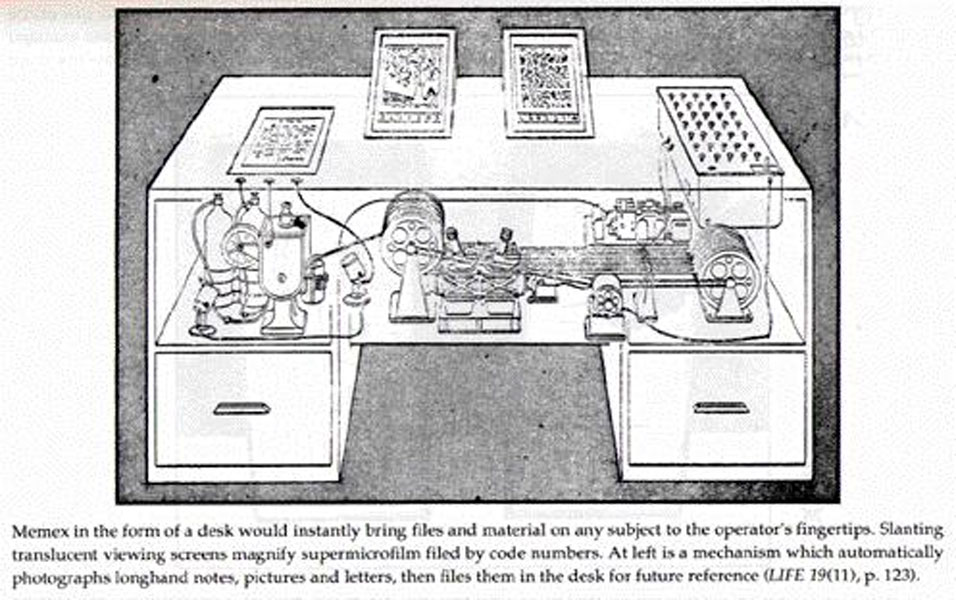
\includegraphics{bush-memex.png}
\caption{Memex machine}
\end{figure}

It consists of a desk, and while it can presumably be operated from a
distance, it is primarily the piece of furniture at which he works. On
the top are slanting translucent screens, on which material can be
projected for convenient reading. There is a keyboard, and sets of
buttons and levers. Otherwise it looks like an ordinary desk.

In one end is the stored material. The matter of bulk is well taken care
of by improved microfilm. Only a small part of the interior of the memex
is devoted to storage, the rest to mechanism. Yet if the user inserted
5000 pages of material a day it would take him hundreds of years to fill
the repository, so he can be profligate and enter material freely.

Most of the memex contents are purchased on microfilm ready for
insertion. Books of all sorts, pictures, current periodicals,
newspapers, are thus obtained and dropped into place. Business
correspondence takes the same path. And there is provision for direct
entry. On the top of the memex is a transparent platen. On this are
placed longhand notes, photographs, memoranda, all sorts of things. When
one is in place, the depression of a lever causes it to be photographed
onto the next blank space in a section of the memex film, dry
photography being employed.

There is, of course, provision for consultation of the record by the
usual scheme of indexing. If the user wishes to consult a certain book,
he taps its code on the keyboard, and the title page of the book
promptly appears before him, projected onto one of his viewing
positions.

Frequently-used codes are mnemonic, so that he seldom consults his code
book; but when he does, a single tap of a key projects it for his use.
Moreover, he has supplemental levers. On deflecting one of these levers
to the right he runs through the book before him, each page in turn
being projected at a speed which just allows a recognizing glance at
each. If he deflects it further to the right, he steps through the book
10 pages at a time; still further at 100 pages at a time. Deflection to
the left gives him the same control backwards.

A special button transfers him immediately to the first page of the
index. Any given book of his library can thus be called up and consulted
with far greater facility than if it were taken from a shelf. As he has
several projection positions, he can leave one item in position while he
calls up another. He can add marginal notes and comments, taking
advantage of one possible type of dry photography, and it could even be
arranged so that he can do this by a stylus scheme, such as is now
employed in the telautograph seen in railroad waiting rooms, just as
though he had the physical page before him.

\textbf{Associative indexing}\\
All this is conventional, except for the projection forward of
present-day mechanisms and gadgetry. It affords an immediate step,
however, to associative indexing, the basic idea of which is a provision
whereby any item may be caused at will to select immediately and
automatically another. This is the essential feature of the memex. The
process of tying two items together is the important thing.

When the user is building a trail, he names it, inserts the name in his
code book, and taps it out on his keyboard. Before him are the two items
to be joined, projected onto adjacent viewing positions. At the bottom
of each there are a number of blank code spaces, and a pointer is set to
indicate one of these on each item. The user taps a single key, and the
items are permanently joined. In each code space appears the code word.
Out of view, but also in the code space, is inserted a set of dots for
photocell viewing; and on each item these dots by their positions
designate the index number of the other item.

Thereafter, at any time, when one of these items is in view, the other
can be instantly recalled merely by tapping a button below the
corresponding code space. Moreover, when numerous items have been thus
joined together to form a trail, they can be reviewed in turn, rapidly
or slowly, by deflecting a lever like that used for turning the pages of
a book. It is exactly as though the physical items had been gathered
together from widely separated sources and bound together to form a new
book. It is more than this, for any item can be joined into numerous
trails.

The owner of the memex, let us say, is interested in the origin and
properties of the bow and arrow. Specifically he is studying why the
short Turkish bow was apparently superior to the English long bow in the
skirmishes of the Crusades. He has dozens of possibly pertinent books
and articles in his memex. First he runs through an encyclopedia, finds
an interesting but sketchy article, leaves it projected. Next, in a
history, he finds another pertinent item, and ties the two together.
Thus he goes, building a trail of many items. Occasionally he inserts a
comment of his own, either linking it into the main trail or joining it
by a side trail to a particular item. When it becomes evident that the
elastic properties of available materials had a great deal to do with
the bow, he branches off on a side trail which takes him through
textbooks on elasticity and tables of physical constants. He inserts a
page of longhand analysis of his own. Thus he builds a trail of his
interest through the maze of materials available to him.

And his trails do not fade. Several years later, his talk with a friend
turns to the queer ways in which a people resist innovations, even of
vital interest. He has an example, in the fact that the outraged
Europeans still failed to adopt the Turkish bow. In fact he has a trail
on it. A touch brings up the code book. Tapping a few keys projects the
head of the trail. A lever runs through it at will, stopping at
interesting items, going off on side excursions. It is an interesting
trail, pertinent to the discussion. So he sets a reproducer in action,
photographs the whole trail out, and passes it to his friend for
insertion in his own memex, there to be linked into the more general
trail.

\textbf{Wholly new forms}\\
Wholly new forms of encyclopedias will appear, ready made with a mesh of
associative trails running through them, ready to be dropped into the
memex and there amplified. The lawyer has at his touch the associated
opinions and decisions of his whole experience, and of the experience of
friends and authorities. The patent attorney has on call the millions of
issued patents, with familiar trails to every point of his client's
interest. The physician, puzzled by a patient's reactions, strikes the
trail established in studying an earlier similar case, and runs rapidly
through analogous case histories, with side references to the classics
for the pertinent anatomy and histology. The chemist, struggling with
the synthesis of an organic compound, has all the chemical literature
before him in his laboratory, with trails following the analogies of
compounds, and side trails to their physical and chemical behavior.

\hypertarget{how-google-search-works}{%
\section{How Google search works}\label{how-google-search-works}}

\emph{Vannevar Bush dreamed of a ``mesh of associative trails'' and of
``associative indexing'' that would help users navigate information
structures. That mesh is now a web--}the web. \emph{Sergey Brin and
Larry Page indexed that web when they created Google. They weren't the
first to index the web, but they did conceive an algorithm that provided
better results than any other search engine.}

\emph{The video and reading below should help you understand why }links
\emph{are so crucial to any web content creator. The video comes from
Google's
\href{https://www.google.com/search/howsearchworks/crawling-indexing/}{How
Search Works} page, while the reading comes from
\href{http://infolab.stanford.edu/~backrub/google.html}{The Anatomy of a
Large-Scale Hypertextual Web Search Engine}, a paper Brin and Page wrote
as Stanford graduate students.}

\textbf{How search works}\\
Pay special attention to the importance of Google's ``PageRank'' formula
at about 1:30.

\begin{center}\rule{0.5\linewidth}{\linethickness}\end{center}

\textbf{From ``The Anatomy of a Large-Scale Hypertextual Web Search
Engine'' by Sergey Brin and Lawrence Page (1998)}

The Google search engine has two important features that help it produce
high precision results. First, it makes use of the link structure of the
Web to calculate a quality ranking for each web page. This ranking is
called PageRank and is described in detail in {[}Page 98{]}. Second,
Google utilizes link to improve search results.

\textbf{PageRank: Bringing Order to the Web}\\
The citation (link) graph of the web is an important resource that has
largely gone unused in existing web search engines. We have created maps
containing as many as 518 million of these hyperlinks, a significant
sample of the total. These maps allow rapid calculation of a web page's
``PageRank'', an objective measure of its citation importance that
corresponds well with people's subjective idea of importance. Because of
this correspondence, PageRank is an excellent way to prioritize the
results of web keyword searches. For most popular subjects, a simple
text matching search that is restricted to web page titles performs
admirably when PageRank prioritizes the results (demo available at
google.stanford.edu). For the type of full text searches in the main
Google system, PageRank also helps a great deal.

\textbf{Description of PageRank Calculation}\\
Academic citation literature has been applied to the web, largely by
counting citations or backlinks to a given page. This gives some
approximation of a page's importance or quality. PageRank extends this
idea by not counting links from all pages equally, and by normalizing by
the number of links on a page. PageRank is defined as follows:

\begin{quote}
We assume page A has pages T1\ldots{}Tn which point to it (i.e., are
citations). The parameter d is a damping factor which can be set between
0 and 1. We usually set d to 0.85. There are more details about d in the
next section. Also C(A) is defined as the number of links going out of
page A. The PageRank of a page A is given as follows:

PR(A) = (1-d) + d (PR(T1)/C(T1) + \ldots{} + PR(Tn)/C(Tn))

Note that the PageRanks form a probability distribution over web pages,
so the sum of all web pages' PageRanks will be one.
\end{quote}

\textbf{Intuitive Justification}\\
PageRank can be thought of as a model of user behavior. We assume there
is a ``random surfer'' who is given a web page at random and keeps
clicking on links, never hitting ``back'' but eventually gets bored and
starts on another random page. The probability that the random surfer
visits a page is its PageRank. And, the d damping factor is the
probability at each page the ``random surfer'' will get bored and
request another random page. One important variation is to only add the
damping factor d to a single page, or a group of pages. This allows for
personalization and can make it nearly impossible to deliberately
mislead the system in order to get a higher ranking. We have several
other extensions to PageRank, again see {[}Page 98{]}.

Another intuitive justification is that a page can have a high PageRank
if there are many pages that point to it, or if there are some pages
that point to it and have a high PageRank. Intuitively, pages that are
well cited from many places around the web are worth looking at. Also,
pages that have perhaps only one citation from something like the Yahoo!
homepage are also generally worth looking at. If a page was not high
quality, or was a broken link, it is quite likely that Yahoo's homepage
would not link to it. PageRank handles both these cases and everything
in between by recursively propagating weights through the link structure
of the web.

\textbf{Anchor Text}\\
The text of links is treated in a special way in our search engine. Most
search engines associate the text of a link with the page that the link
is on. In addition, we associate it with the page the link points to.
This has several advantages. First, anchors often provide more accurate
descriptions of web pages than the pages themselves. Second, anchors may
exist for documents which cannot be indexed by a text-based search
engine, such as images, programs, and databases. This makes it possible
to return web pages which have not actually been crawled. Note that
pages that have not been crawled can cause problems, since they are
never checked for validity before being returned to the user. In this
case, the search engine can even return a page that never actually
existed, but had hyperlinks pointing to it. However, it is possible to
sort the results, so that this particular problem rarely happens.

This idea of propagating anchor text to the page it refers to was
implemented in the World Wide Web Worm {[}McBryan 94{]} especially
because it helps search non-text information, and expands the search
coverage with fewer downloaded documents. We use anchor propagation
mostly because anchor text can help provide better quality results.
Using anchor text efficiently is technically difficult because of the
large amounts of data which must be processed. In our current crawl of
24 million pages, we had over 259 million anchors which we indexed.

\textbf{Other Features}\\
Aside from PageRank and the use of anchor text, Google has several other
features. First, it has location information for all hits and so it
makes extensive use of proximity in search. Second, Google keeps track
of some visual presentation details such as font size of words. Words in
a larger or bolder font are weighted higher than other words. Third,
full raw HTML of pages is available in a repository.

\hypertarget{dark-patterns}{%
\section{Dark Patterns}\label{dark-patterns}}

\emph{Dark patterns are design strategies used by content developers to
trick you into taking some action you wouldn't otherwise take. You have
certainly encountered dark patterns before, but you (a) may not have
recognized them as manipulative or (b) may not have realized that these
patterns are indeed patterns--once you recognize them, you'll see
variations all over the web.}

\emph{Check out the video below and then visit the
\href{https://darkpatterns.org/}{Dark Patterns} website.}

\hypertarget{buzzfeeds-formula}{%
\section{Buzzfeed's formula}\label{buzzfeeds-formula}}

\emph{This article is from 2014, which is in some respects a long time
ago. But the core insights of
\href{http://tubularinsights.com/buzzfeed-video-formula/}{Buzzfeed's
video formula}, excerpted below, will still resonate with most anyone
who has ever blown a couple hours taking Buzzfeed quizzes.}

\emph{Of particular note are Buzzfeed's ``pillars of content'':
``emotional gift,'' ``information,'' and ``identity.'' These pillars
ensure that Buzzfeed creates not just consumable content, but } sharable
\emph{content.}

\begin{figure}
\centering
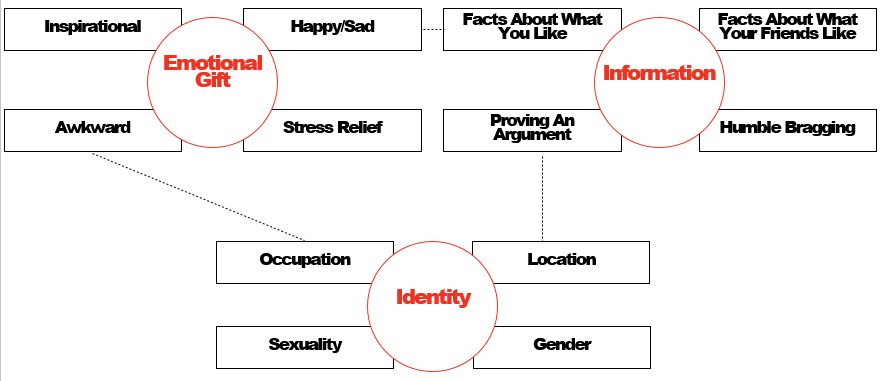
\includegraphics{buzzfeed-content-categories.png}
\caption{Buzzfeed content categories}
\end{figure}

\textbf{Emotional Gift:} This type of content taps into the vast range
of human emotions. A BuzzFeed video should be able to change your mood
from a sad to a happy one, it should be able to relieve stress, and give
the viewer respite from upsetting personal, or even world events. The
whole point of the video content is to make the viewer feel something --
if they feel it, they will share it.

\textbf{Information:} Can you present information in a new, interesting
way? Never underestimate the power of the humble brag -- give the viewer
the impression that they were aware of most of the facts, but were
genuinely happy to learn a couple more. Also, great informational videos
can help prove or disprove an argument, and that makes them
fantastically shareable.

\textbf{Identity:} This is huge, and demonstrated by just how popular
the BuzzFeed quizzes are. People want to to be identified as something,
to belong to a group, and taking the BuzzFeed quizzes is one way of
confirming where they belong. Or not, in some cases. But it's all good
because it all leads to that content being shared.

\hypertarget{atom}{%
\chapter{Atom}\label{atom}}

\hypertarget{introducing-atom}{%
\section{Introducing Atom}\label{introducing-atom}}

\textbf{\href{https://atom.io/}{Atom}} is a text editor. A text editor
is a little bit like Microsoft Word, but for coding. With a little setup
and practice, however, you may find yourself writing your English papers
in Atom instead of Word. Atom is faster, simpler, prettier, and does
most of what you need in terms of text production. At the very least,
it's \emph{much} better than Word for taking notes and writing things
for the internet.

We'll eventually use it to code websites, but first we'll use it for
writing blog posts. So let's install it and customize it for those
tasks.

This process might be a little scary, but do the best you can. I'll
include some links to help you if you get stuck.

\hypertarget{installing-atom}{%
\section{Installing Atom}\label{installing-atom}}

First, let's install the program and put it where it belongs on your
computer.

\begin{enumerate}
\def\labelenumi{\arabic{enumi}.}
\tightlist
\item
  If you don't have \textbf{Google Chrome} on your computer,
  \href{https://support.google.com/chrome/answer/95346?co=GENIE.Platform\%3DDesktop\&hl=en}{download}
  it. You don't \emph{technically} need Chrome, but it's what we'll use
  to examine code later in the semester.
\item
  Open Chrome and go to \href{https://atom.io/}{atom.io}. You should see
  a screen like the one below.\\
  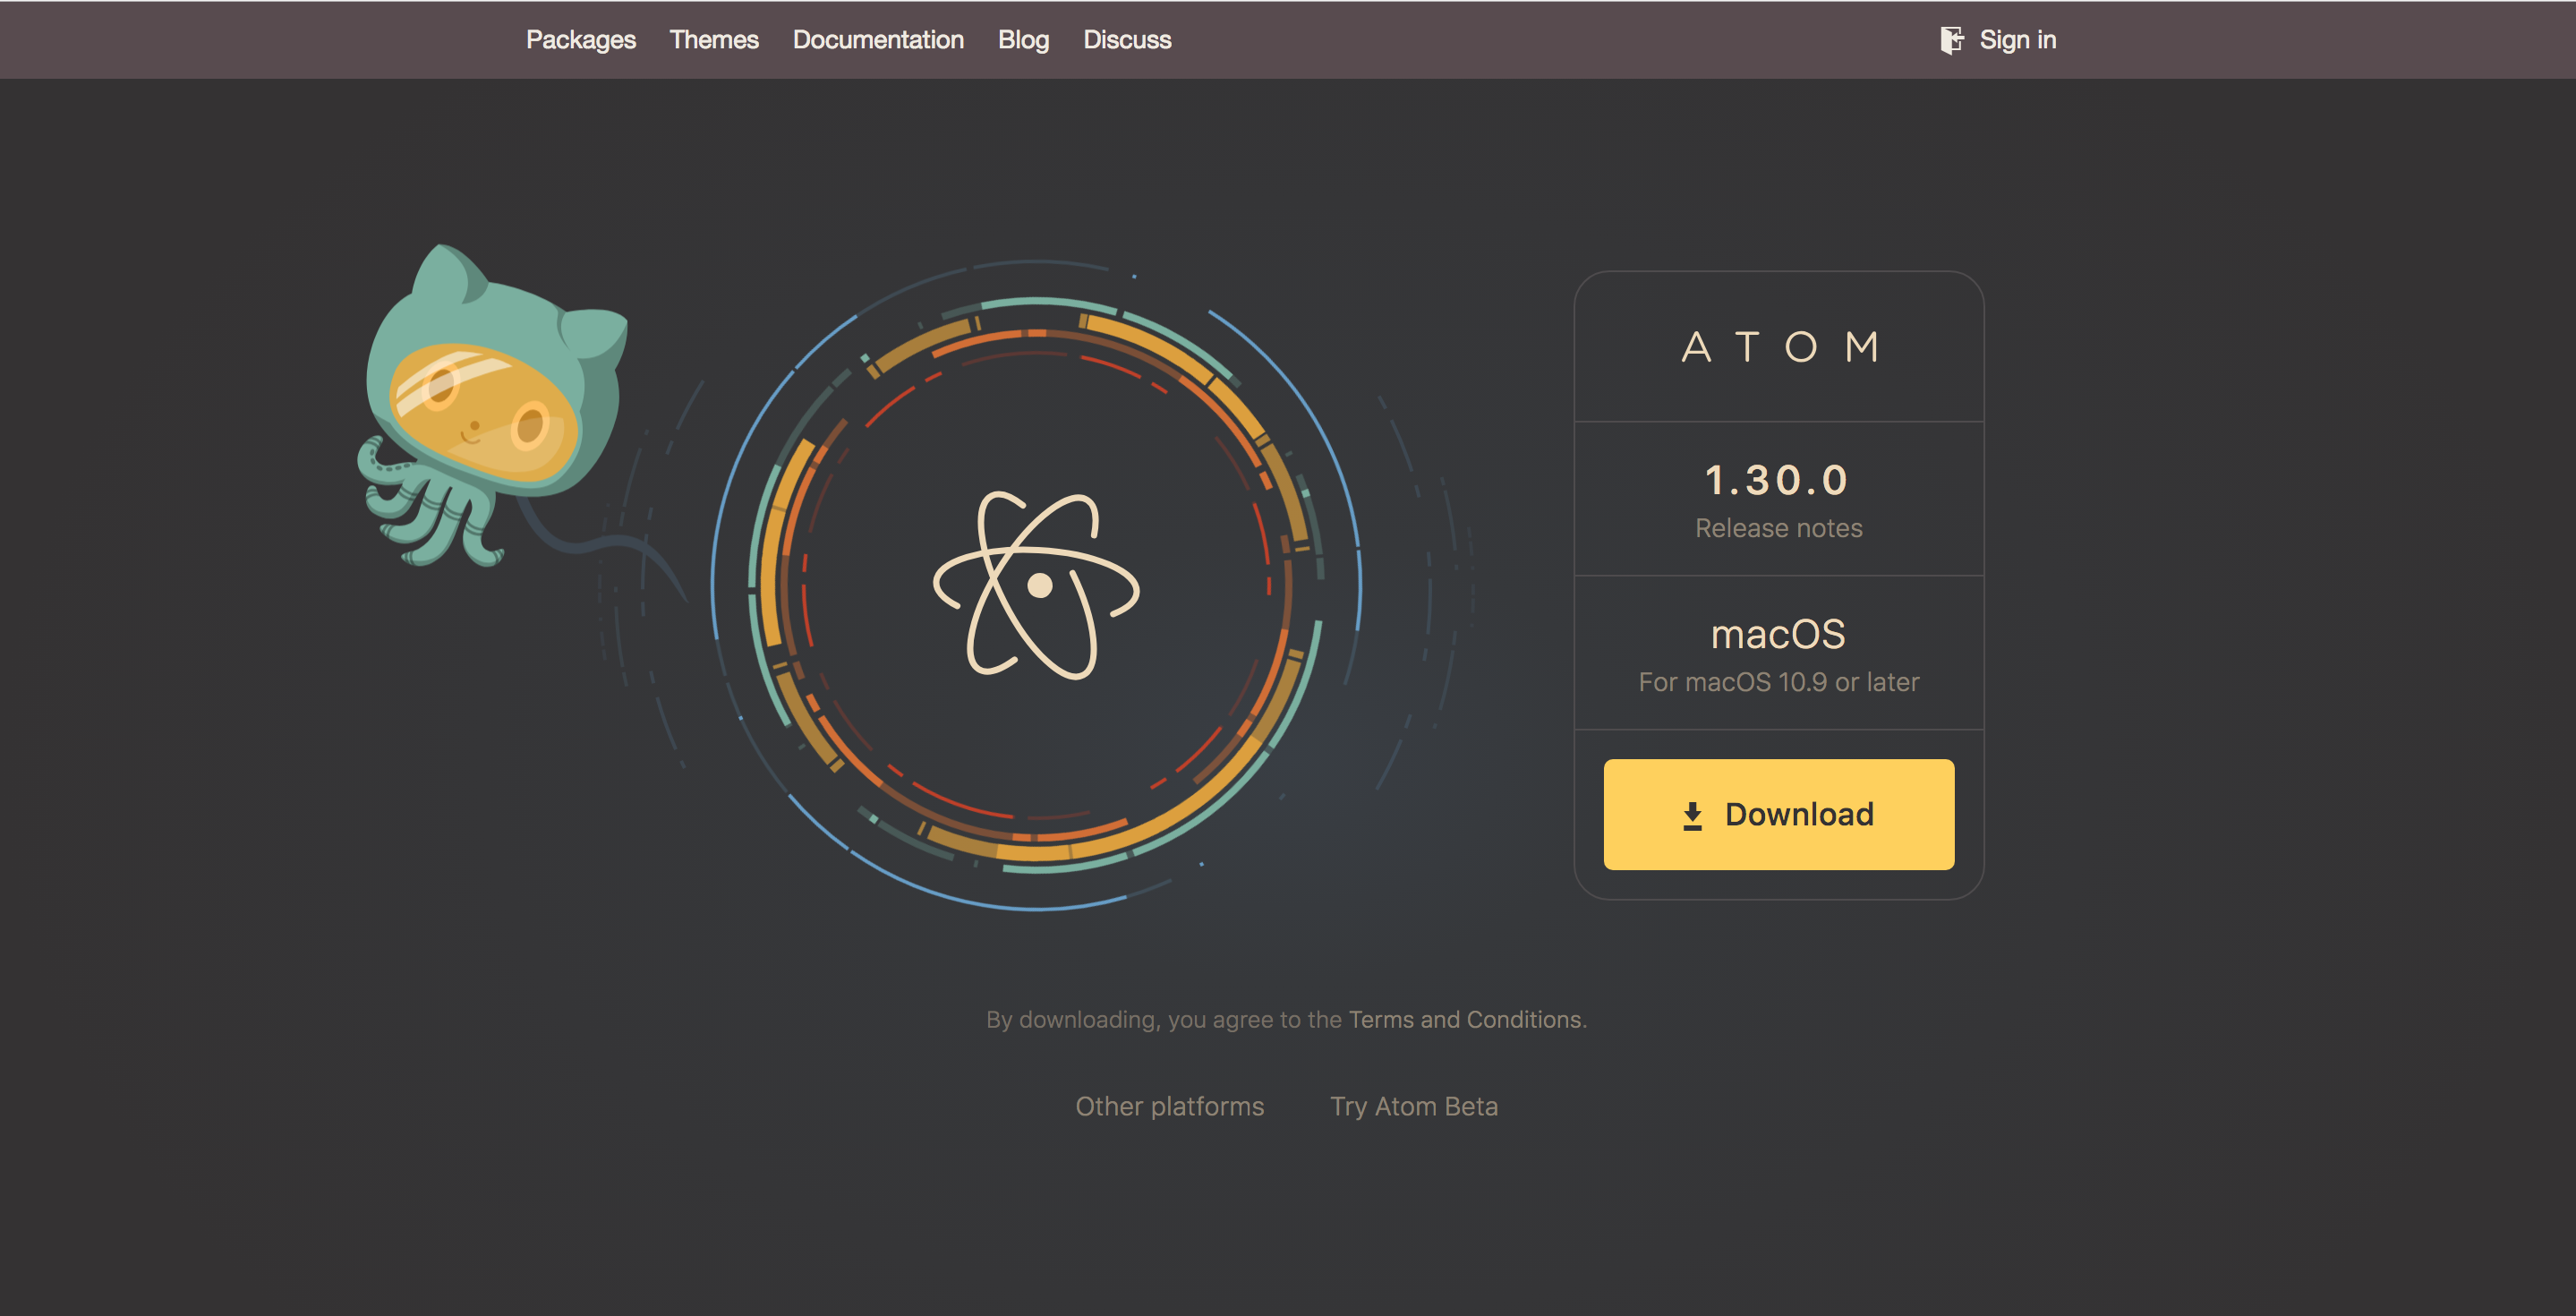
\includegraphics{atom-getting-started.png}
\item
  See the \textbf{Download} button? Click it. Your computer should then
  download a .zip (Mac) or .exe (Win) file. Some computers may
  automatically open and unpack the .zip file. If yours doesn't, then
  open the .zip file yourself. (If you don't know how to open .zip files
  on your computer, Google it.) Eventually, you should see the Atom
  icon.
\item
  If you're using a Mac, drag that icon to your \textbf{Applications}
  folder. If you're using Windows, Atom should automatically add an Atom
  shortcut to your \textbf{desktop} and your \textbf{Start menu}.~
\item
  Click the Atom icon to launch Atom!
\end{enumerate}

For more info/help, visit the
\href{http://flight-manual.atom.io/getting-started/sections/installing-atom/\#platform-mac}{Installing
Atom} section of the Atom documentation. Note that at the top of the
page you can choose your operating system (Windows or Mac).

\hypertarget{setting-up-atom-and-installing-packages}{%
\section{Setting up Atom and installing
packages}\label{setting-up-atom-and-installing-packages}}

Atom's a little different than Word. Word comes with a whole bunch of
features, most of which you'll never use. Atom comes with a few features
but allows you to quickly install many more. You install those features
via the \textbf{package manager}. Let's install most of the packages
we'll need this semester. While we're at it, we'll adjust some other
settings to make Atom a more comfortable writing environment.

\begin{enumerate}
\def\labelenumi{\arabic{enumi}.}
\tightlist
\item
  Once you've launched Atom, you should see a screen with a Welcome
  Guide and other information. At the top of the screen, you should see
  a menu bar like you do with other applications (File, Edit, View,
  etc.). Open the Settings view by choosing \textbf{File =\textgreater{}
  Settings (Win)} or \textbf{Atom =\textgreater{} Preferences (Mac)}.
  Alternatively, if you want to be a baller, just hit \textbf{ctrl+comma
  (Win)} or \textbf{cmd+comma (Mac)}. You should see a screen like the
  one below.\\
  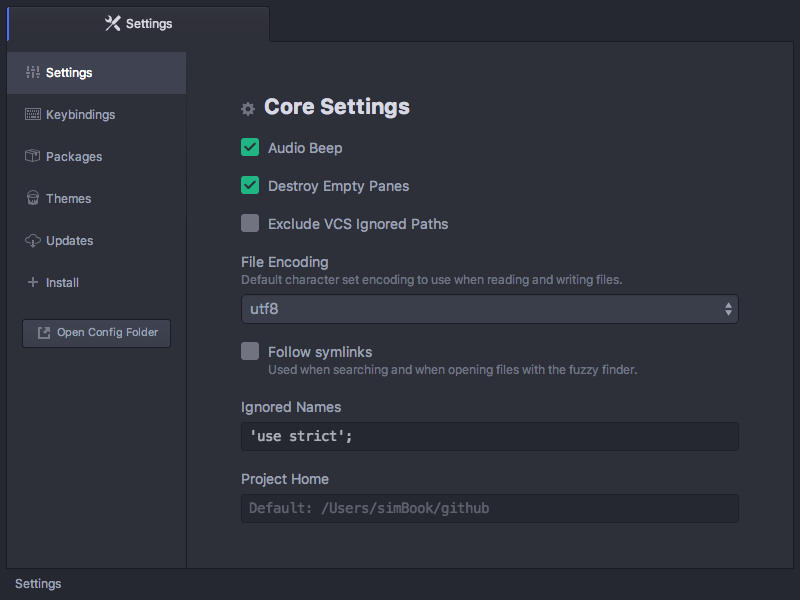
\includegraphics{atom-settings.png}
\item
  First, click the Editor tab, scroll down to \textbf{Soft Wrap}, and
  check the corresponding box.
\item
  Next, click the Themes tab. Here you can choose a dark background or a
  light background. If you prefer a dark background, do nothing. If you
  prefer a light background, choose One Light. Be sure to change both
  the UI Theme and the Syntax Theme.
\item
  Finally, click the Install tab. You should see a screen like the one
  below.\\
  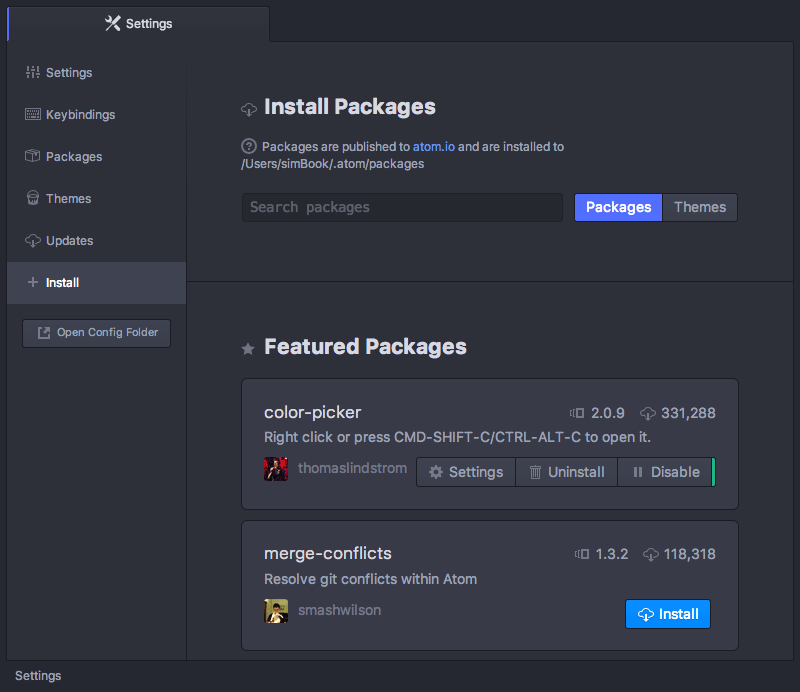
\includegraphics{packages-install.png}
\item
  In the Install Packages search bar, search for \textbf{atom-beautify}.
  When the package appears, click the \textbf{Install} button and wait
  for the installation to complete. Congrats--you've just installed a
  package!
\item
  Repeat step 5 for each of the packages below. Once you've installed
  the packages, you can view some of them in the Packages menu (in the
  same menu bar as File, Edit, View, etc.).

  \begin{itemize}
  \tightlist
  \item
    \textbf{atom-html-preview} -- allows you to view changes to your
    website from within Atom
  \item
    \textbf{emmet} -- allows you to write your code more quickly
  \item
    \textbf{linter} -- helps identify potential errors in your code.
    When you install this one, Atom may ask you to install
    ``dependencies.'' Allow each of these
  \item
    \textbf{markdown-writer} -- allows you to make pretty documents with
    no fuss (we'll use this one right away!)
  \item
    \textbf{tool-bar} -- with the next package, adds a toolbar with
    buttons for italics, etc.
  \item
    \textbf{tool-bar-markdown-writer} -- see directly above
  \item
    \textbf{pandoc-convert} -- converts Markdown files (see below) to
    Word docs, PDFs, or other formats
  \end{itemize}
\end{enumerate}

\hypertarget{optional-packages}{%
\section{Optional packages}\label{optional-packages}}

If you wish, you may also download these packages:

\begin{itemize}
\tightlist
\item
  \textbf{wordcount} -- adds a word count to the bottom of Atom's
  interface
\item
  \textbf{linter-write-good} -- tries to identify common writing issues
  (e.g., passive voice). Can be helpful, but when in doubt use your own
  judgment.
\end{itemize}

\hypertarget{command-palette}{%
\section{Command Palette}\label{command-palette}}

You can do pretty much anything in Atom--open files, install packages,
convert files from one type to another--via the Command Palette. To open
the palette, type \textbf{cmd+shift+p} (Mac) or \textbf{ctrl+shift+p}
(Win).

Now type whatever you want to do (e.g., open file, change theme, spell
check) and select the option you want. At first you may struggle to
figure out the right thing to type, but after some practice, using the
Command Palette will be much faster than clicking through the various
menus and submenus (though you can always do that, too!).

\hypertarget{markdown}{%
\chapter{Markdown}\label{markdown}}

Markdown is a lightweight markup language, which basically means that it
allows you to easily create italics, boldface, links, images, and
bulleted/numbered lists. Markdown is faster than Word for most kinds of
writing, but the best part is that a Markdown file can become a Word
doc, a PDF, an HTML file, a slide show, an MLA document--whatever!

You can find a Markdown tutorial at
\href{https://commonmark.org/help/tutorial/}{CommonMark}.

\hypertarget{create-a-markdown-file}{%
\section{Create a Markdown file}\label{create-a-markdown-file}}

Make your first Markdown file in Atom by following the steps below.

\begin{enumerate}
\def\labelenumi{\arabic{enumi}.}
\item
  In Atom, choose \textbf{File =\textgreater{} New file.}
\item
  Save the file as a Markdown file by choosing \textbf{File
  =\textgreater{} Save.} Name the file markdown-test.md. Be sure to use
  the \textbf{.md} suffix.
\item
  Paste the text below into the file, then save the file.

\begin{verbatim}
# This is a heading 1 element  
This is a paragraph. To make a paragraph break, just leave an extra line of space.  

This is a new paragraph.  

* This is a list item  
* So is this  

## This is a heading 2 element  
1. Here's a numbered list item  
2. And a **bold** item  
3. And an *italics* item  
4. And a [link](http://www.google.com)
\end{verbatim}
\item
  Now, to see the output, look for the Packages menu in the menu bar
  (File, Edit, View, etc.) at the top of the screen. Click Packages,
  then choose Markdown Preview. You should see a preview window like the
  one below.\\
  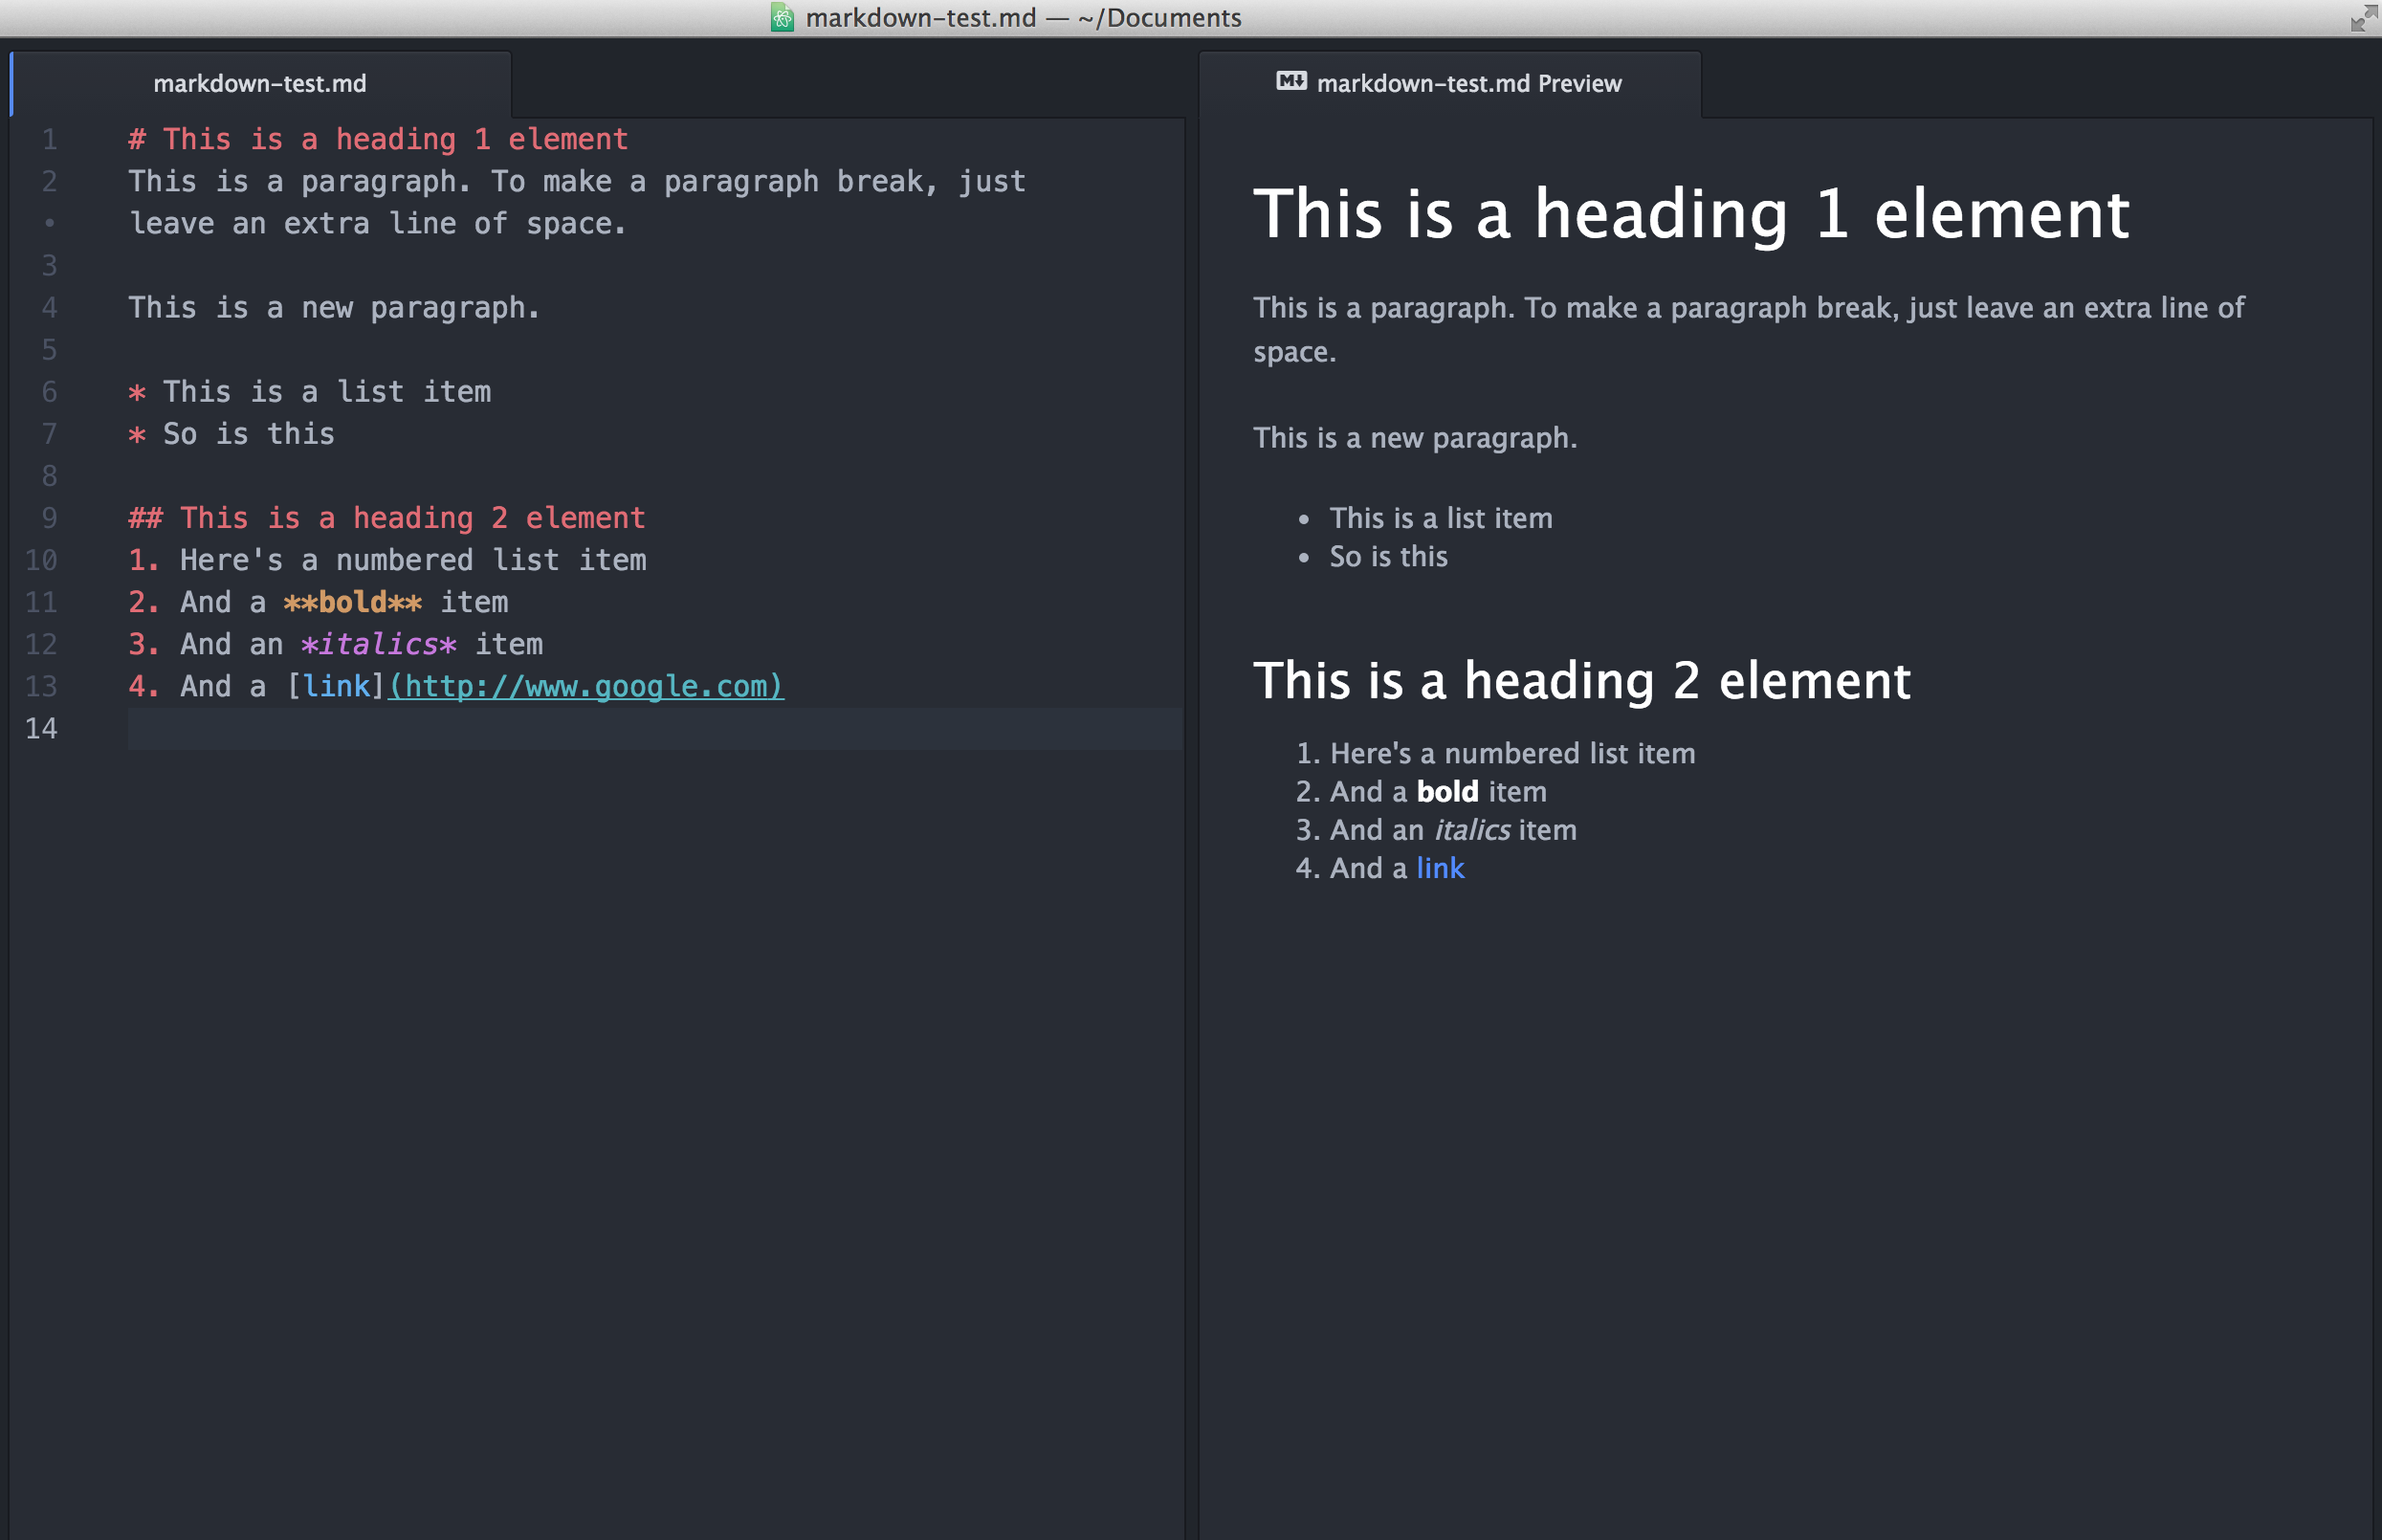
\includegraphics{markdown.png}
\item
  That's it! Markdown is that simple. If you want to learn more, use the
  \href{https://guides.github.com/pdfs/markdown-cheatsheet-online.pdf}{Markdown
  cheat sheet}. Soon, we'll learn how to convert Markdown to a nice pdf
  or html document--and how to paste perfectly formatted writing into
  emails, newsletters, Google or Word docs, and more.
\end{enumerate}

\hypertarget{convert-markdown-to-html-word-or-pdf-formats}{%
\section{Convert Markdown to HTML, Word, or PDF
formats}\label{convert-markdown-to-html-word-or-pdf-formats}}

Markdown's greatest feature is that Markdown content can become pretty
much any other kind of content. Your Markdown can become a web page, a
Word doc, a PDF, an MLA paper, an ebook (like this one!), a
slideshow--whatever.

\textbf{HTML}\\
HTML is the language of most web pages. Generally, each web page on a
site consists of a single \texttt{.html} file. To convert your Markdown
into HTML,

\begin{enumerate}
\def\labelenumi{\arabic{enumi}.}
\tightlist
\item
  In \href{https://andylaut.github.io/3844-guidebook/atom.htm}{Atom},
  make sure you're viewing your Markdown file. Open Markdown Preview by
  selecting \textbf{Packages =\textgreater{} Markdown Preview
  =\textgreater{} Toggle Preview.}
\item
  Right-click some blank space in the preview window and select
  \textbf{Save As HTML}. Atom will give you the options of renaming your
  file and selecting a save location. Be sure the filename ends in
  \texttt{.html} (if you see something like \texttt{filename.md.html},
  you can delete the \texttt{.md} part). Save it to your documents
  folder (or wherever).
\item
  Find your new HTML file on your computer, and double-click it to open
  it in your web browser. If you want to view or edit the HTML file,
  simply open it in Atom!
\end{enumerate}

\textbf{Pasting HTML into Medium}\\
In most cases, you can paste your HTML into Medium with no errors.
Simply open the HTML file in your browser (step 3 above), then copy the
entire document to your clipboard. Paste the copied content into the
Medium editor.

\textbf{Word or PDF}\\
To convert your Markdown to Word or PDF format, you'll need Atom's
\textbf{pandoc-convert} package. See
\href{https://andylaut.github.io/3844-guidebook/atom.html\#setting-up-atom-and-installing-packages}{\textbf{Setting
up Atom and installing packages}}. To convert your Markdown,

\begin{enumerate}
\def\labelenumi{\arabic{enumi}.}
\tightlist
\item
  In \href{https://andylaut.github.io/3844-guidebook/atom.htm}{Atom},
  make sure you're viewing your Markdown file.
\item
  Press \texttt{cmd+shift+p} (Mac) or \texttt{ctrl+shift+p} (Win) to
  open the
  \href{https://andylaut.github.io/3844-guidebook/atom.html\#command-palette}{Command
  Palette}.
\item
  In the Command Palette textbox, type \textbf{pandoc docx} (for Word)
  or \textbf{pandoc pdf} (for PDF). When you see the option you want,
  click the option or press return.
\item
  Atom will give you the options of renaming your file and selecting a
  save location. Be sure the filename ends in \texttt{.docx} or
  \texttt{.pdf} (if you see something like \texttt{filename.md.docx},
  you can delete the \texttt{.md} part). Save it to your documents
  folder (or wherever).
\item
  Find the new Word or PDF doc on your computer and open it!
\end{enumerate}

Some people have reported problems converting to PDF format. You may be
able to fix this problem by downloading LaTeX, a document preparation
system. If you don't anticipate using Markdown outside of this course,
then you can skip this step and simply convert to Word format instead.

\textbf{MLA}\\
Want to acheive perfect MLA formatting every time? Try
\href{http://markdowntomla.com/}{markdowntomla.com}!

You can also use Markdown to make slide decks \emph{way} faster than you
could with PowerPoint. \href{http://deckdown.org/}{Deckdown} is a good
place to start, but once we learn HTML and GitHub, we can add images,
videos, etc.

\hypertarget{cheat-sheet}{%
\section{Cheat sheet}\label{cheat-sheet}}

This cheat sheet comes from Matt Cone at
\href{https://www.markdownguide.org/cheat-sheet/}{markdownguide.org}.
You can also find a cheat sheet within Atom by clicking \textbf{Packages
=\textgreater{} Markdown Writer =\textgreater{} Open Cheat Sheet.}

Element

Markdown Syntax

Atom Shortcut

Heading

\texttt{\#\ H1} \texttt{\#\#\ H2} \texttt{\#\#\#\ H3}

Bold

\texttt{**bold\ text**}

\texttt{b\ tab}

Italic

\texttt{*italicized\ text*}

\texttt{i\ tab}

Blockquote

\texttt{\textgreater{}\ blockquote}

Ordered List

\texttt{1.\ First\ item} \texttt{2.\ Second\ item}
\texttt{3.\ Third\ item}

Unordered List

\texttt{-\ First\ item} \texttt{-\ Second\ item} \texttt{-\ Third\ item}

Code

\texttt{\textasciigrave{}code\textasciigrave{}}

\texttt{code\ tab}

Horizontal Rule

\texttt{-\ -\ -}

Link

\texttt{{[}anchor{]}(https://www.example.com\ "title")}

\texttt{l\ tab}

Image

\texttt{!{[}alt\ text{]}(image.jpg\ "title")}

\texttt{img\ tab}

\hypertarget{medium}{%
\chapter{Medium}\label{medium}}

Medium is part blogging platform, part social network. Like most any
other blogging platform, Medium allows you to post multimedia content.
Unlike some other platforms, however, Medium also lets you follow other
users, mention and link to other users (just like an @ on Twitter or tag
on Facebook or Instagram). You can also follow particular topics (e.g.,
``Education,'' ``JavaScript'') and tag your own content with topics.

\hypertarget{medium-help}{%
\section{Medium help}\label{medium-help}}

Medium offers extensive user documentation. I've copied the links below
from the \href{https://help.medium.com/hc/en-us}{Medium support} page,
where you can also find help on modifying your account settings, sharing
on social media, and much more.

Creating in Medium

 Managing posts

Your drafts \& posts

Your stats

Tags

Share draft

Unlisted publishing

Revision history

Content licenses

 Writing \& editing

Write post

Format text

Images

Embeds

Custom titles \& subtitles

 Partner Program

Join Partner Program

Write for members

Your Partner Program dashboard

Friend Links

Calls to action

 Responses \& notes

Write response

Leave note

 Migrations \& integrations

Import post

Import archive

Wordpress plugin

Publishing API

 Tips \& more

Medium's Curation Guidelines

Update Facebook \& Twitter cards

Keyboard shortcuts

\hypertarget{pasting-markdown-authored-content-into-medium}{%
\section{Pasting Markdown-authored content into
Medium}\label{pasting-markdown-authored-content-into-medium}}

You can compose directly in Medium's editor, but in this class we
compose in Markdown. We use Markdown because Markdown content can become
so many other types of content. (See the
\protect\hyperlink{markdown}{Markdown chapter} of this book.) Composing
in Markdown also ensures that you always have a copy on your own
computer. After all, you never know when you might lose your internet
connection.

To cleanly paste your Markdown-authored content into Medium, you should
first convert your content into an HTML file, then open that HTML file
in your browser, copy the file's contents, then paste into Medium.

\textbf{Converting from Markdown to HTML}\\
To convert your Markdown content to HTML, you can use two methods. If
you have installed the
\href{https://andylaut.github.io/3844-guidebook/atom.html\#setting-up-atom-and-installing-packages}{pandoc}
package, you can convert to HTML the same way you would convert to Word
or any other format:

\begin{enumerate}
\def\labelenumi{\arabic{enumi}.}
\tightlist
\item
  In \href{https://andylaut.github.io/3844-guidebook/atom.htm}{Atom},
  make sure your cursor is in your Markdown file.
\item
  Open the
  \href{https://andylaut.github.io/3844-guidebook/atom.html\#command-palette}{Command
  Palette} by typing \texttt{cmd+shift+p} (Mac) or \texttt{ctrl+shift+p}
  (Win).
\item
  In the text entry field, type ``pandoc html5'' and press
  \texttt{return}.
\item
  Choose the name and path of your file. Make sure your filename ends in
  \texttt{.html} (e.g., \texttt{filename.html}, \textbf{NOT} simply
  \texttt{filename}). If the suggested filename contains the text
  \texttt{.md}, you may delete that text.
\item
  Press \texttt{return}. You should receive confirmation if the process
  succeeds.
\end{enumerate}

If you don't have pandoc, you can follow the alternate instructions
below.

\begin{enumerate}
\def\labelenumi{\arabic{enumi}.}
\tightlist
\item
  In \href{https://andylaut.github.io/3844-guidebook/atom.htm}{Atom},
  make sure you're viewing your Markdown file. Open Markdown Preview by
  selecting \textbf{Packages =\textgreater{} Markdown Preview
  =\textgreater{} Toggle Preview.}
\item
  Right-click some blank space in the preview window and select
  \textbf{Save As HTML}. Atom will give you the options of renaming your
  file and selecting a save location. Be sure the filename ends in
  \texttt{.html} (if you see something like \texttt{filename.md.html},
  you can delete the \texttt{.md} part). Save it to your documents
  folder (or wherever).
\item
  Find your new HTML file on your computer, and double-click it to open
  it in your web browser. If you want to view or edit the HTML file,
  simply open it in Atom!
\end{enumerate}

\textbf{Pasting HTML into Medium}\\
This part is simpler. To paste your HTML into Medium, simply

\begin{enumerate}
\def\labelenumi{\arabic{enumi}.}
\tightlist
\item
  Find the HTML file on your computer and open it in your web browser
  (Chrome recommended).
\item
  Copy the contents of the page to your clipboard.
\item
  Paste the contents of the page into Medium's editor.
\end{enumerate}

In most cases, the content should paste perfectly. Sometimes, however,
you may encounter problems such as

\begin{itemize}
\tightlist
\item
  \textbf{Images don't paste.} If you included an image in your Markdown
  file, it will only paste into Medium if the image was located on the
  web (e.g., on Google Images, NOT on your computer). To add an image
  that IS located on your computer, see the
  \href{https://help.medium.com/hc/en-us/articles/215679797}{Medium Help
  Center}.
\item
  \textbf{Headings look different.} Medium offers two levels of
  headings, no more. If you try to include additional levels of
  headings, Medium will change your formatting. Use only two levels of
  headings.
\item
  \textbf{Just straight-up didn't work.} You may have converted your
  file incorrectly, pasted incorrectly, or written invalid or
  too-complicated Markdown. See me for help.
\end{itemize}

\hypertarget{using-images-resources-and-fair-use-guidelines}{%
\section{Using images: resources and fair use
guidelines}\label{using-images-resources-and-fair-use-guidelines}}

The internet unlocked access to more content than any of us could ever
consume. Anyone with a fast enough connection can download software,
videos, podcasts, blogs, and of course images.

While much of this content is freely available, U.S. intellectual
property laws apply even to free content--including images. Contrary to
popular belief, using someone else's image violates the law in most
cases, even if you acknowledge the source.

The U.S. Copyright Office's
\href{https://www.copyright.gov/fair-use/more-info.html}{fair use
guidelines} includes four criteria for judging fair use of intellectual
property:

\begin{itemize}
\tightlist
\item
  \textbf{Purpose and character of the use, including whether the use is
  of a commercial nature or is for nonprofit educational purposes.}
  Nonprofit use is more likely to be considered fair, and so is
  transformative use (i.e., use that adds something new and doesn't
  substitute for the original use). However, nonprofit use is NOT
  necessarily fair use.
\item
  \textbf{Nature of the copyrighted work.} Use of news or documentary
  content is more likely to be considered fair than use of ``creative''
  content like novels or songs.
\item
  \textbf{Amount and substantiality of the portion used in relation to
  the copyrighted work as a whole}. Use of small portions is more likely
  to be considered fair. However, despite what you may have heard, there
  is no ``10\% rule.''
\item
  \textbf{Effect of the use upon the potential market for or value of
  the copyrighted work}. The less impact the use has on the value of the
  copyrighted work, the more likely it is that the use will be
  considered fair.
\end{itemize}

Keep these myths in mind:

\begin{itemize}
\tightlist
\item
  You do NOT necessarily have the right to use someone else's images (or
  other content) just because you acknowledge the creator.
\item
  You do NOT necessarily have the right to use up to 10\% (or any other
  specific amount) of someone else's work.
\item
  Educational use is NOT necessarily fair use.
\end{itemize}

\begin{figure}
\centering
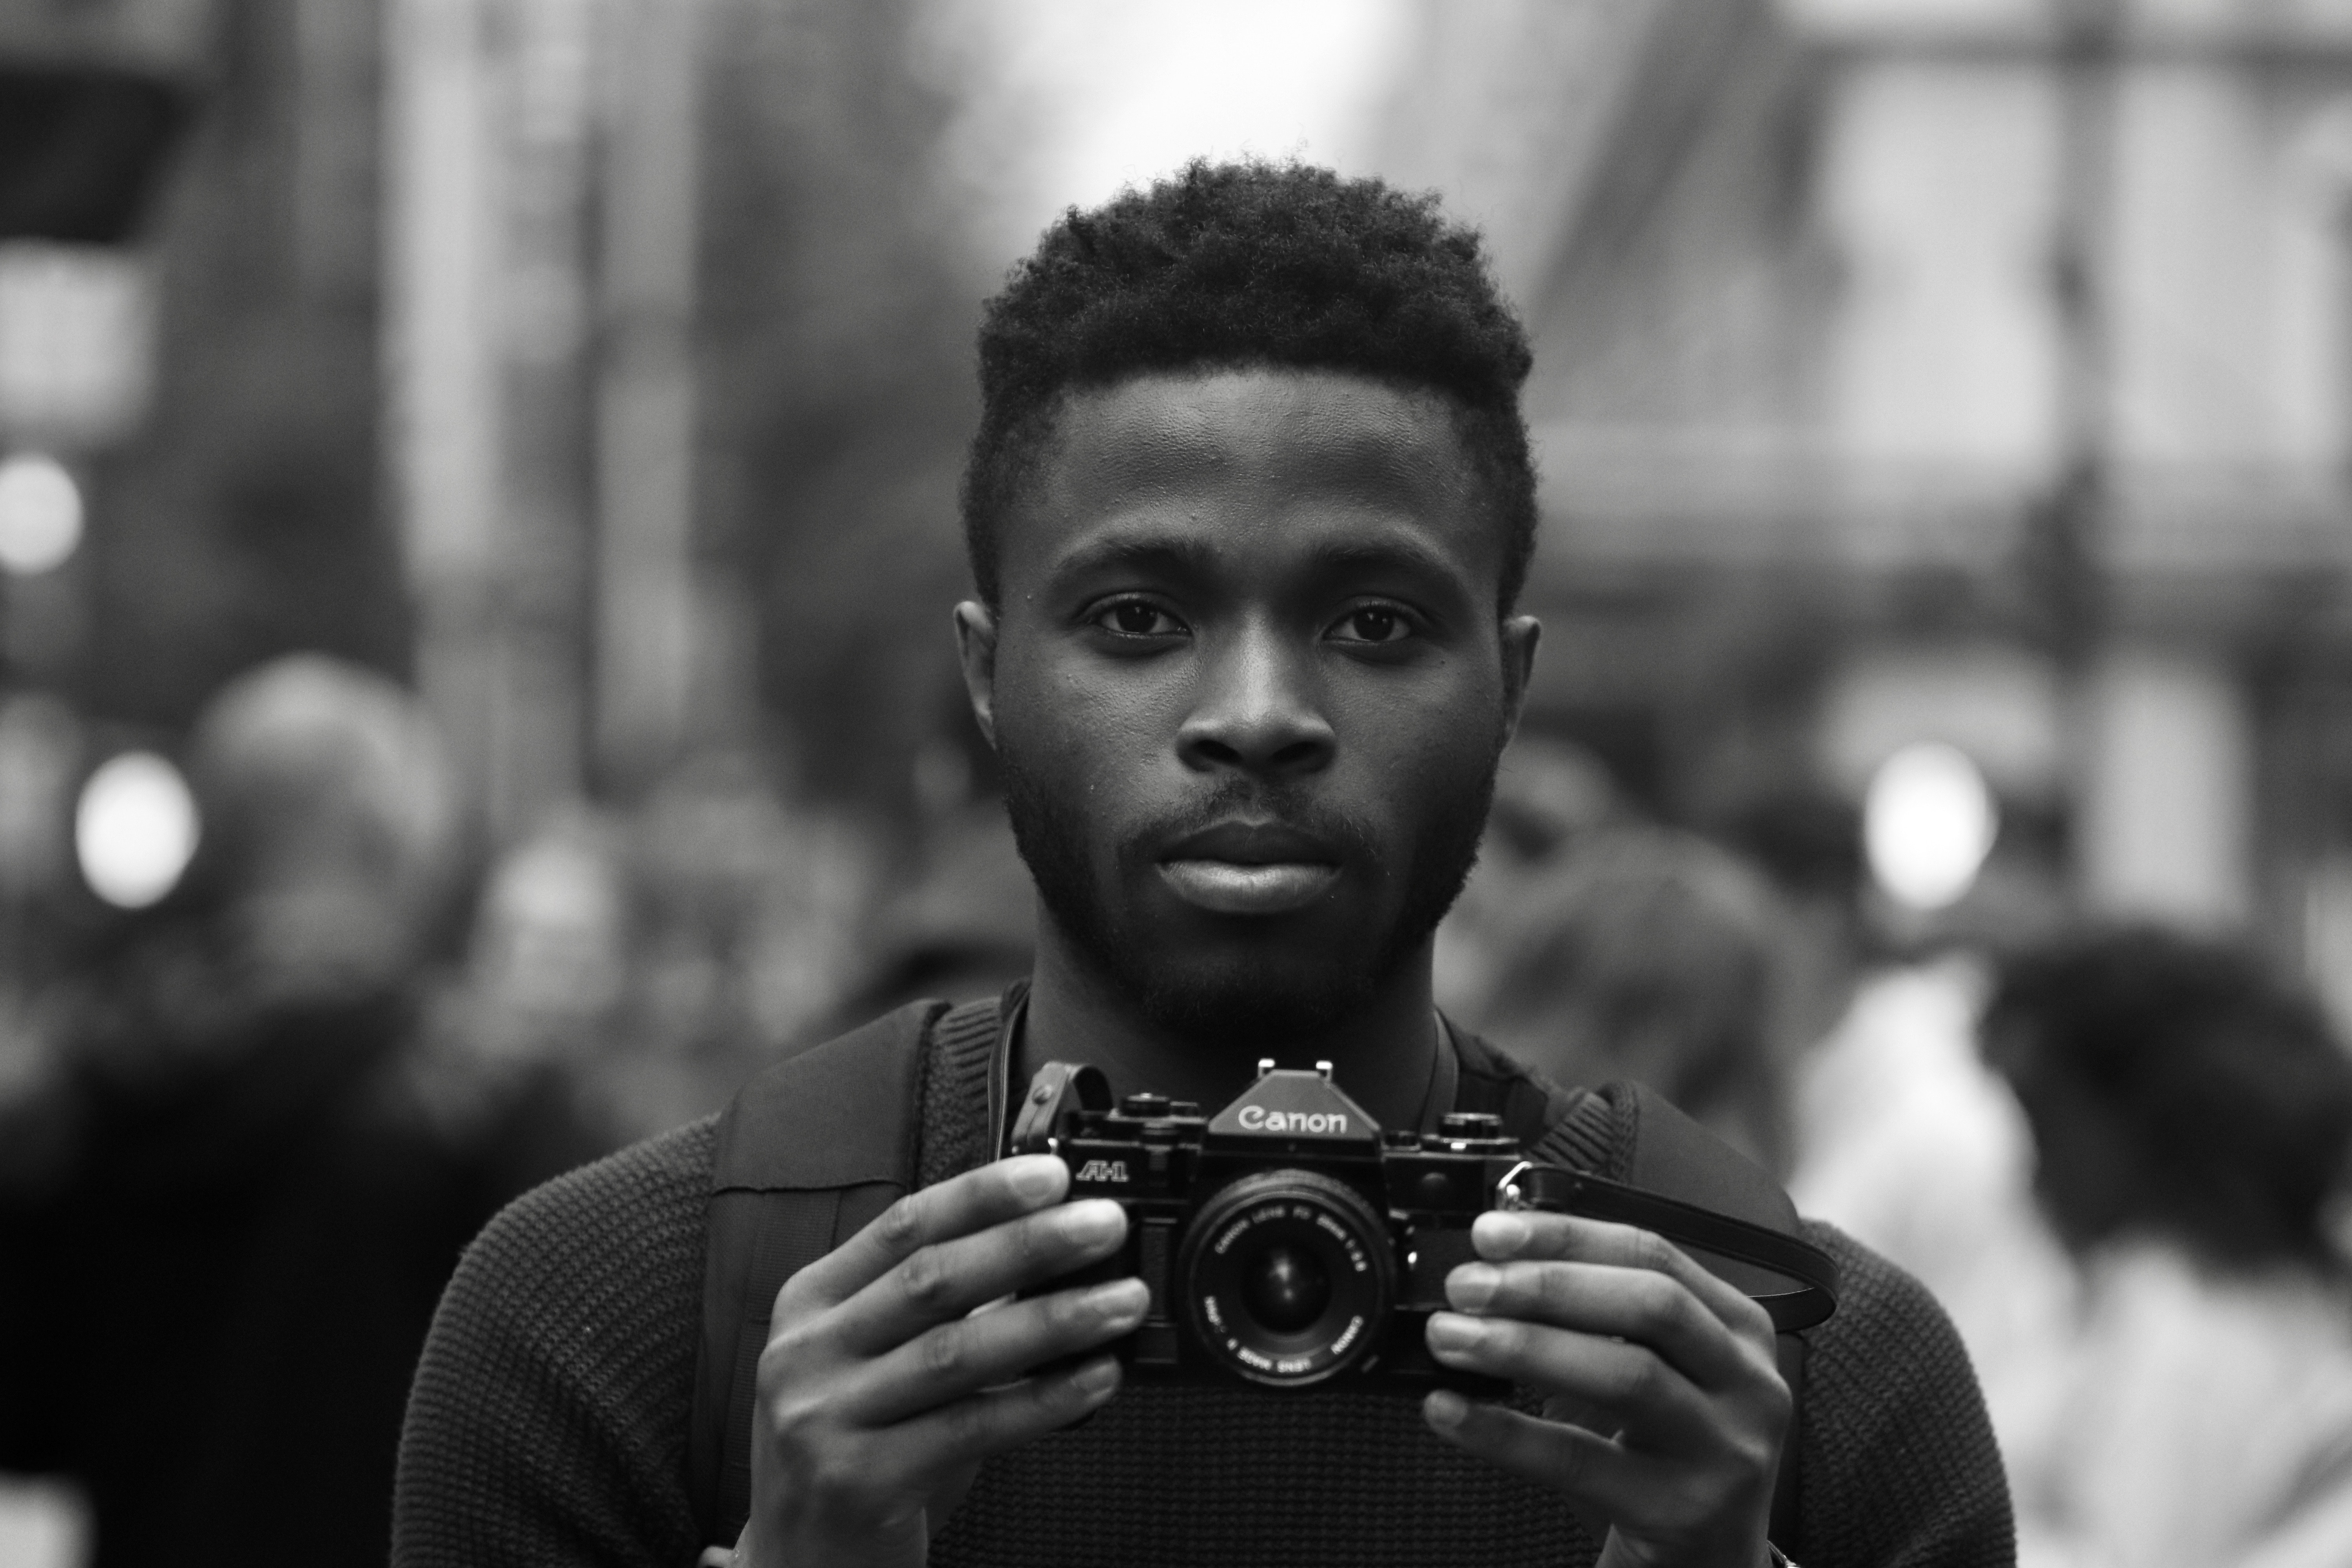
\includegraphics{dimitri-de-vries.jpg}
\caption{Photo by Dimitri de Vries on Unsplash}
\end{figure}

\textbf{Free and legal image resources}\\
Fortunately, you can find freely usable images if you know where to
look. Google Images actually has a
\href{https://support.google.com/websearch/answer/29508?hl=en}{usage
rights search filter}, though the quality of the results can vary, as
can the constraints on usage.

One way to determine which usage constraints apply is to use only
\href{https://search.creativecommons.org/}{Creative Commons}-licensed
images. Creative Commons licenses clearly define the terms of fair use
for a given image (or other content type). You can read more about
license types on Creative Commons's
\href{https://creativecommons.org/licenses/}{licenses} page.

But if you want to be extra safe AND find reliably high-quality photos,
the sites below exclusively offer Creative Commons Zero (CC0)-licensed
photographs. A CC0 license entitles you to use licensed content freely
and without attribution (though attribution is still good manners).

\begin{itemize}
\tightlist
\item
  \textbf{\href{https://unsplash.com/}{Unsplash}.} Unsplash offers CC0
  photos, but they do encourage you to provide attribution--and they
  make attribution easy. See an example above.
\item
  \textbf{\href{https://pixabay.com/}{Pixabay}.} Pixabay offers CC0
  photos, illustrations, and video clips.
\end{itemize}

\hypertarget{emmet-html-shortcuts}{%
\chapter{Emmet HTML shortcuts}\label{emmet-html-shortcuts}}

HTML is the language of the web. In many ways, HTML is a blessing: It
allows creators across the world to make consistent, clear, usable
content. Nevertheless, writing in HTML can feel like a chore. (How many
times do I have to type
\texttt{\textless{}p\textgreater{}\textless{}/p\textgreater{}}?)
\textbf{Emmet} makes HTML easy--easier, in fact, than writing similar
documents in Word--assuming those documents contain headings, links,
images, lists, etc.

Emmet provides an extensive list of shortcuts for HTML, CSS, and more.
You can find the full list via the
\href{https://docs.emmet.io/cheat-sheet/}{Emmet cheatsheet}, but here's
a table of some of the handiest Emmet shortcuts.

Content

Shortcut

Result

HTML doc

!

\texttt{\textless{}!DOCTYPE\ html\textgreater{}\ (document\ skeleton)}\\

Link

a

\texttt{\textless{}a\ href=""\textgreater{}\textless{}/a\textgreater{}}

Image

img

\texttt{\textless{}img\ src=""\ alt=""\ /\textgreater{}}

Bold

str

\texttt{\textless{}strong\textgreater{}\textless{}/strong\textgreater{}}

Italics

em

\texttt{\textless{}em\textgreater{}\textless{}/em\textgreater{}}\\

Ordered (numbered) list

ol+

\texttt{\textless{}ol\textgreater{}\ \ \ \ \ \ \ \ \ \ \ \ \ \textless{}li\textgreater{}\textless{}/li\textgreater{}\ \ \ \ \ \ \ \ \ \textless{}/ol\textgreater{}}\\

Unordered (bulleted) list

ul+

\texttt{\textless{}ul\textgreater{}\ \ \ \ \ \ \ \ \ \ \ \ \ \ \ \ \ \textless{}li\textgreater{}\textless{}/li\textgreater{}\ \ \ \ \ \ \ \ \ \ \ \ \ \textless{}/ul\textgreater{}}\\

You can always add HTML content by converting Markdown to HTML.

Create an HTML document in Atom.

Open your Markdown file in Atom.

Open the Markdown Preview window and right-click.

Select Copy as HTML.

Paste your HTML into the appropriate place (probably somewhere in the
body section) in your HTML document

\bibliography{book.bib,packages.bib}


\end{document}
